\documentclass{article}

%% Page Margins %%
\usepackage{geometry}
\geometry{
    top = 0.75in,
    bottom = 0.75in,
    right = 0.75in,
    left = 0.75in,
}

\usepackage{amsmath}
\usepackage{graphicx}
\usepackage{parskip}
\usepackage{amssymb}
\usepackage{enumerate}

\title{Assembly Project: Dr Mario}

\author{Areez Chishtie}

\begin{document}
\maketitle

\section{Demo Details}

\begin{enumerate}[(I)]

\item How to view the game:

\begin{itemize}
\item Display width in pixels: \texttt{64}
\item Display height in pixels: \texttt{64}
\item Unit width in pixels: \texttt{2}
\item Unit height in pixels: \texttt{2}
\item Base Address for display: \texttt{0x10008000 (\$gp)}
\end{itemize}

\item How to play the game:

\begin{itemize}
\item To move the pill, use '\texttt{a}', \texttt{d}', and '\texttt{s}'.
\item To rotate the pill clockwise, use '\texttt{w}'. Note that the pill "stays in place" during rotations, so it may appear as though only two out of the four orientations of the pill are supported, but if you press '\texttt{w}' twice, the colours of the pills will have swapped.
\item To save/restore the pill (easy feature \#15), use '\texttt{e}'. If a pill is currently stored, it is visible on the right, below the four upcoming pills in the queue.
\item To pause/resume the game, press '\texttt{p}'.
\item To quit the game, press '\texttt{q}'.
\item The game includes sound effects, to remember to turn on sound!
\end{itemize}

\begin{figure}[ht!]
\centering
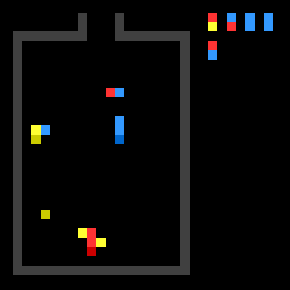
\includegraphics[width=0.3\textwidth]{Images/game.png}
\caption{A screenshot of the game in progress. On the right, the four upper pills depict the queue of upcoming pills (with the leftmost one being the very next pill), and the one lower pill represents the saved pill.}
\label{fig:game}
\end{figure}

\end{enumerate}

\section{Implementation Details}

\begin{enumerate}[(I)]

\item Which milestones were implemented? 

All milestones (1--5) are implemented. For milestones 4--5, I implemented 8 easy features:
\begin{itemize}
\item[1.] Basic gravity.
\item[2.] The speed of gravity doubles after half of the viruses have been eliminated.
\item[5.] Sound effects on: game start/reset/next-level, landing a pill, pause/resume, rotating the pill, eliminating a line, and upon eliminating half of the viruses (to signal the enhanced gravity stage)
\item[6.] Game pause/resume upon pressing '\texttt{p}'. I chose to draw a pause symbol ($\shortparallel$) instead of writing 'Pause'.
\item[7.] A level system that scales the total number of viruses. The number of viruses starts at 4, and increases by 2 every time a level is completed.
\item[11.] A panel on the side displays a preview of the next capsule in queue.
\item[12.] The panel is augmented to display the next 4 capsules in queue.
\item[15.] The player can save/restore the current pill by pressing '\texttt{e}'.
\end{itemize}

\item Summary of the implementation:

\begin{itemize}
\item Initially, four viruses are randomly positioned and coloured in the lower half of the playing field. If two viruses happen to be randomized to the same location, a new random location is generated for one of them. (This can technically fall into an "infinite" loop, but I decided that accounting for this is unnecessary given the spirit of this project.) The colours of the viruses are darker than their corresponding pill colours, for visual clarity as well as the ability to distinguish between them in code.
\item The current pill, queue of next pills, and saved pill are all stored into arrays in memory using similar representations. Each pill is made up of two pixels whose colours (and possibly positions) are maintained in memory.
\item I decided to mostly stick with bitmap coordinates when making computations, as this makes it easier to draw things to the display. Sometimes it was simpler to work in Cartesian coordinates (i.e., when randomizing virus locations, or determining the orientation of the current pill), so I implemented \texttt{cart\_to\_bitm} and \texttt{bitm\_to\_cart} functions.
\item When the player maneuvers the current pill, collision detection isn't handled directly through the display bitmap, but rather through another bitmap in memory that I called \texttt{field}. This is a replica of the display bitmap that consists only of objects which the current pill can collide with, namely, the medicine bottle and all already-fallen static pills. Also, this allowed me to draw the medicine bottle only once to \texttt{field}, instead of having to re-compute it every iteration of the game loop.
\item The most complex part of the game is checking for lines of four or more same-colour pixels, eliminating them, then allowing any unsupported pixels to drop. This is all handled by the \texttt{eliminate\_field} function, which calls the helper function \texttt{eliminate\_line}. The helper function searches one vertical or horizontal line of the playing field from end to end, and eliminates any same-colour lines of four or more. It also counts how many viruses appeared in the eliminated line segment, and reduces the total virus count (in memory) accordingly.
\item Whenever the player lands the current pill somewhere, \texttt{eliminate\_field} is called. It in turn calls \texttt{eliminate\_line} once on every vertical and horizontal line of the playing field, and then runs an asynchronous game loop that searches \texttt{field} bottom-up for any unsupported pixels, and drops them by one pixel each iteration until all pixels are supported.
\end{itemize}

\end{enumerate}

\end{document}